\documentclass[12pt]{article}
\usepackage[portuguese]{babel}
\usepackage[utf8]{inputenc}
\usepackage[usenames,dvipsnames]{color}
\usepackage{setspace}
\usepackage{amsmath}
\usepackage{amsfonts}
\usepackage{amssymb}
\usepackage{mathtools}
\usepackage[top=3cm, bottom=2cm, left=3cm, right=2cm]{geometry}
\usepackage{tikz}
\usepackage{indentfirst}
\usepackage{textcomp}
\usepackage{float}
\usepackage[font={small,it}]{caption}
\usepackage{mhchem}
\title{Relatorio Parcial Mestrado}

% packages added by Marcelo
%
\usepackage{lscape}    % for landscape pages
\usepackage{hyperref}  % to allow hyperlinks
\usepackage{booktabs}  % nicer table borders
\usepackage{subfigure} % add subfigures

% My default commands
\newcommand{\foreignword}[1]{\textit{#1}}
\newcommand{\toolname}[1]{\textit{#1}}
%\newcommand{\fieldR}{\mathbb{R}}
\newcommand{\powerset}{\mathcal{P}}
%\newcommand{\probability}{\mathbb{P}}
\newcommand{\expectation}{\mathbb{E}}
\newcommand{\algname}[1]{\texttt{#1}}
\newcommand{\langname}[1]{\texttt{#1}}
%\newcommand{\varname}[1]{\texttt{#1}}
%\newcommand{\floor}[1]{\lfloor #1 \rfloor}
%\newcommand{\ceil}[1]{\lceil #1 \rceil}
%\newcommand{\mathsc}[1]{{\normalfont\textsc{#1}}}
\newcommand{\forest}{\mathcal{F}}
\newcommand{\pfsnode}[1]{\mathbf #1}
\newcommand{\species}[1]{\textit{#1}}
\newcommand{\gender}[1]{\textit{#1}}

\graphicspath{{./img/}} 

\setstretch{1.5}

\begin{document}

% FAPESP demands the usage of double spacing
%
\doublespacing

\begin{titlepage}
    \vfill 
    \begin{center}
        {\Large Relatório Científico Parcial -- Mestrado\\
         \bigskip
         Processo FAPESP 17/20575-9
        }
        
        \bigskip
        \bigskip
    
        {\LARGE Identificação de vias de sinalização celular baseada em repositórios de cinética de reações bioquímicas}

        \bigskip
        \bigskip
        {\Large {\bf Beneficiário:} \href{mailto:gustavo.estrela.matos@usp.br}{Gustavo Estrela de Matos}\\ 
        
        {\bf Responsável:} \href{mailto:marcelo.reis@butantan.gov.br}{Marcelo da Silva Reis}\\

        \bigskip
        \bigskip
        \bigskip
        \bigskip
        \bigskip
        \bigskip
        \bigskip
Relatório referente aos trabalhos desenvolvidos entre 1 de janeiro e 10 de dezembro de 2018

        \bigskip
        \bigskip
        \bigskip
        \bigskip
        \bigskip
        \bigskip
        \bigskip

Laboratório Especial de Toxinologia Aplicada, Instituto Butantan\\
        \bigskip
        São Paulo, \today\\
        }

        \bigskip
        \bigskip

       

\end{center}
\end{titlepage}


\tableofcontents

\pagebreak



\section{Resumo do Projeto Proposto} \label{sec:resumo} % até 2 páginas
A construção de modelos funcionais é uma técnica comum para se 
estudar vias de sinalização celular e, quando a via estudada é pouco
conhecida, é possível que os modelos já propostos sejam incompletos, 
tornando necessário a sua modificação.
Lulu Wu apresentou em 2015, em sua dissertação de mestrado, um método 
para  modificar sistematicamente modelos funcionais, adicionando a estes
interações extraídas de repositórios como KEGG. Entretanto, esta 
metodologia apresentou limitações: a primeira é a incompletude do banco 
de dados de interações criado, que extraia informações apenas do 
repositório KEGG; a segunda, a falta de informações sobre constantes 
de velocidade de interações, que podem ser extraídas de repositórios 
como BioNumbers; a terceira, a dinâmica do algoritmo de busca, 
incremental, que pode não achar o mínimo global; e a última, a 
penalização na complexidade dos modelos, que era feita de maneira 
aleatória. Propomos neste trabalho enfrentar as limitações encontradas
pela metodologia de Lulu, criando um banco de dados de interações mais
completo e também novas funções de custo que sejam capazes de 
penalizar modelos mais complexos (como critério de informação Akaike e 
{\em Bayesian inference-based modeling}); esta penalização deve induzir,
em cadeias do  espaço de busca, curvas em u no custo dos modelos, 
portanto também propomos a criação de novos algoritmos de busca que 
explorem essa característica da função de custo. Por fim, esperamos 
testar nossa metodologia na identificação de vias de sinalização celular 
da linhagem tumoral murina Y1.

\section{Introdução}
% Uma introdução enxuta do projeto, com outline e objetivos.
Vias de sinalização celular podem ser simuladas por modelos dinâmicos
computacionais e, mais especificamente, modelos que descrevem a 
concentração de espécies químicas ao longo do tempo são chamados de 
modelos funcionais. Neste projeto, trabalhamos com modelos funcionais
que descrevem as mudanças de concentrações de espécies químicas através
de equações diferenciais ordinárias (EDOs). Estes modelos, quando não 
sofrem de sobreajuste (\foreignword{overfitting}), se tornam 
interessantes quando são capazes de reproduzir dados observados em 
experimentos biológicos, pois dão a estes modelos a qualidade preditiva.

% Agora falamos do problema de identificação de via de sinalização
% celular.
% Quebramos o problema em duas partes:
% 1. Determinar a topologia da via de sinalização
% 2. Determinar constantes de velocidades de interações
% Propomos solucionar os dois problemas retirando dados de bancos de 
% dados de biologia. Mais especificamente, em uma de nossas metodologias 
% propostas tratamos constantes de velocidade como parâmetros aleatórios 
% do sistema, o que dignifica nossa abordagem como Bayesiana.

% Depois falamos que por muitas vezes um mapa estático pode não ter uma
% topologia compatível com o experimento biológico em questão (pode ser
% que falte ou sobre interações). Por isso, torna-se necessário 
% modificar de maneira sistemática. Propomos então neste projeto 
% transformar o problema de identificação de vias de sinalização celular
% em um problema de otimização.

O problema de criar modelos funcionais capazes de explicar resultados
de experimentos biológicos com o mínimo de sobreajuste é chamado de 
{\em problema de identificação de vias de sinalização celular}. Podemos 
separar este problema em duas etapas principais. A primeira diz respeito
a escolha da topologia da via de sinalização, o que é equivalente a 
escolher quais interações químicas são relevantes para o experimento em
questão. A segunda etapa consiste em escolher valores para os parâmetros
do sistema de EDOs do modelo funcional; estes valores são constantes de 
velocidade de interações e/ou concentrações iniciais de espécies 
químicas.

Em casos em que o experimento biológico ou a via de sinalização são 
muito estudadas, é possível que ambas as etapas descritas anteriormente
possam ser resolvidas com pesquisas na literatura. Em casos que isto não
é possível, torna-se uma solução recorrer a bancos de dados de biologia,
para guiar a escolha de interações e constantes do modelo funcional.
Para a primeira etapa, podemos consultar bancos como o 
\href{http://www.genome.jp/kegg/}{Kyoto Encyclopedia of Genes and Genomes (KEGG)}
~\cite{Kanehisa2000kegg}, que contém mapas estáticos; e para a segunda,
podemos consultar bancos como o 
\href{https://www.ebi.ac.uk/biomodels-main/}{BioModels}~\cite{le2006biomodels}
.

Entretanto, os mapas estáticos disponíveis nestes bancos podem ainda ser
incompletos ou muito grandes para o experimento biológico em questão. 
Desta maneira, torna-se importante criar uma maneira sistemática de se
modificar modelos funcionais a fim de faze-los explicar o experimento 
biológico sem sobreajuste. Propomos fazer estas modificações tratando
o problema de identificação de vias de sinalização como um problema de
otimização combinatória, considerando como espaço de busca possíveis 
topologias para o modelo funcional, de acordo com interações retiradas 
de repositórios de biologia e armazenadas em um banco de dados local,
e usando como função de custo alguma métrica que represente a qualidade 
deste modelo ao reproduzir o experimento biológico de interesse.

Considere $S$ um conjunto de interações químicas. O conjunto de todas
as possíveis escolhas de interações relevantes em $S$ corresponde ao
conjunto potência de $S$, $\powerset(S)$, que é o espaço de busca do
problema de otimização que estamos interessados. Se chamamos a nossa 
métrica de qualidade de modelo funcional de $c$, transformamos nosso 
problema em uma instância do problema de seleção de características. 
Assim, após definida a função de custo $c$ e devidamente coletado e 
armazenado o conjunto $S$, propomos resolver instâncias do problema de 
identificação de vias de sinalização celular no arcabouço 
{\em featsel} ~\cite{Reis2017featsel}. A 
figura~\ref{fig:problem_lattice} mostra um exemplo de problema de 
seleção de modelos e o espaço de busca do respectivo problema de seleção
de características equivalente.

\begin{figure}[H]
  \centering 
  \begin{tabular}{c c}
    \subfigure[] {\scalebox{0.3}{
     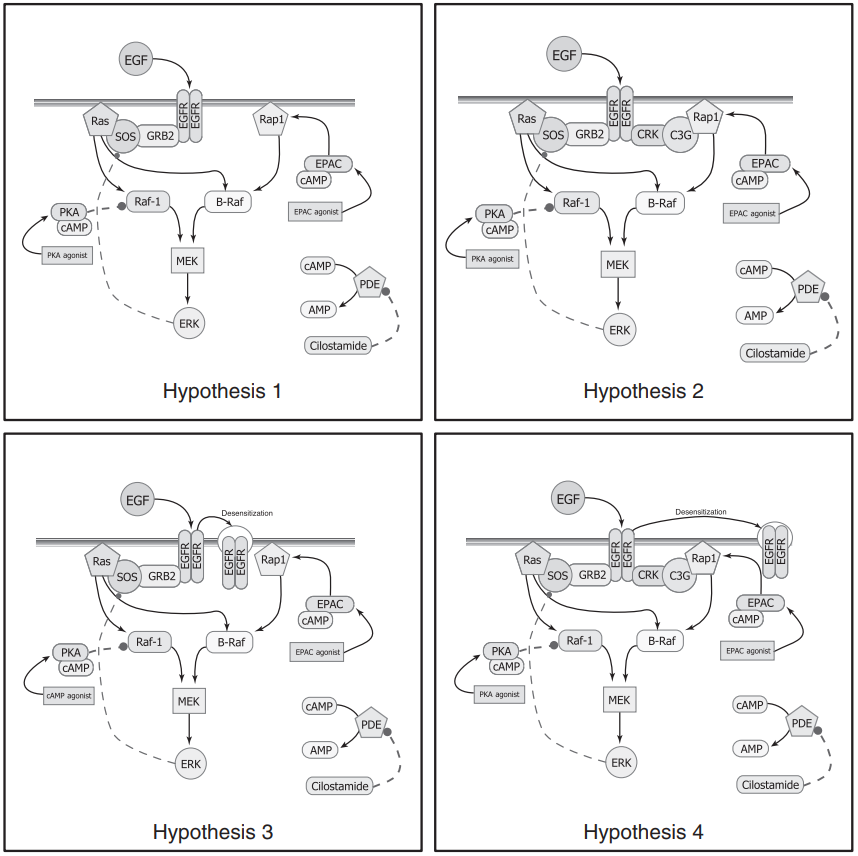
\includegraphics[clip=true]{model_hypothesis.png}}
     \label{fig:model_hypothesis} }
     &
    \subfigure[] {\scalebox{.8}{
    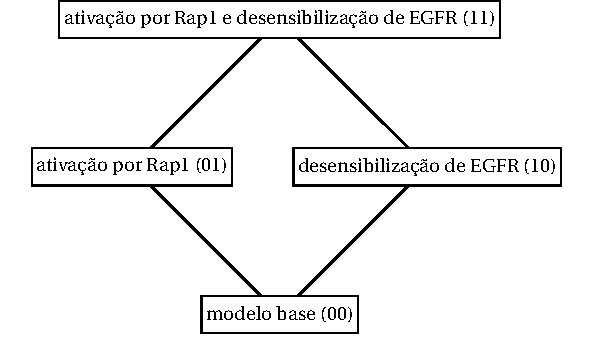
\includegraphics[clip=true]{models_lattice.pdf}}
    \label{fig:hypothesis_lattice} }
  \end{tabular}
    \caption{Exemplo de problema de identificação de via de sinalização
    e o espaço de busca que o representa. Na 
    figura~\ref{fig:model_hypothesis} temos um exemplo de problema de 
    seleção de modelos com 4 modelos; a hipótese 1 pode ser considerada
    como um modelo base pois todos os outros modelos contém as suas 
    interações; a hipótese 2 é igual a hipótese 1 adicionando a ativação
    de ERK por Rap1; a hipótese 3 é igual a hipótese 1 adicionando a 
    desensibilização de EGFR; por fim, a hipótese 4 é igual a hipótese 1
    com ativação de ERK por Rap1 e com desensibilização de EGFR. A 
    figura~\ref{fig:hypothesis_lattice} mostra o espaço de busca da 
    instância de seleção de características que pode ser criada para
    resolver o problema original de seleão de modelos. A 
    figura~\ref{fig:model_hypothesis} foi retirada de~\cite{Xu2010}}
  \label{fig:problem_lattice} 
\end{figure}

\section{Atividades Realizadas}
Nesta seção descrevemos as atividades desenvolvidas durante o período
de início da bolsa até o dia de entrega deste relatório. Na 
seção~\ref{disciplinas} apresentamos as disciplinas cursadas pelo 
beneficiário. Na seção~\ref{model_sel} apresentamos a métrica utilizada
para avaliação de modelos funcionais, $p (D | M)$, que decidimos 
utilizar, e também explicamos a complexidade em seu cálculo analítico. 
Na seção~\ref{estudos_de_estimadores} apresentamos uma técnica 
desenvolvida por Friel e Pettit~\cite{Friel2008} que permite estimar 
esta probabilidade que usamos como métrica com  conceitos de 
termodinâmica. Na seção~\ref{bibm_implementation} descrevemos a 
implementação do SigNetMS, um software que é capaz de calcular de 
estimar a probabilidade $p (D | M)$ utilizando a técnica de 
termodinâmica e algoritmos de geração de amostras com cadeias de Markov.
Por fim, apresentamos resultados de experimentos feitos com o SigNetMS
na seção~\ref{experimentos}.

\subsection{Disciplinas cursadas}\label{disciplinas}
% Mencionar as três matérias feitas
% 1 Tópicos em análise de algoritmos
%   - complementar a análise de algoritmo
% 2 Probabilidade e Inferência Estatística I
% 3 Laboratório de Programação Extrema
% 4 Como ouvinte, aulas de Introdução à Transdução de Sinais 
%   Celulares (Instituto de Química - Universidade de São Paulo)
% 5 Mencionar a matéria do Ronaldo (?)

Durante o período de março a dezembro de 2018, foram cursadas pelo
beneficiários três disciplinas. No primeiro semestre, 
\begin{itemize}
    \item{Tópicos em Análise de Algoritmos:} nesta disciplinas são
        abordadas técnicas para análise de algoritmos e para solução
        de problemas. Muitos problemas abordados nesta disciplina são
        de otimização combinatória, assim como o problema de seleção de 
        características, que propomos utilizar neste projeto.
    \item{Probabilidade e Inferência Estatística I:} esta disciplina
        faz parte do departamento de Estatística do Instituto de 
        Matemática e Estatística (IME-USP). A disciplina é dividida em
        dois módulos: o primeiro módulo aborda probabilidade, enquanto
        o segundo aborda inferência estatística, tanto do ponto de vista
        clássico quanto do ponto de vista Bayesiano. Esta disciplina
        foi necessária para que o beneficiário pudesse entender as 
        duas funções de custo propostas para este trabalho: {\em 
        Akaike's Information Criterion}, uma abordagem clássica; e 
        {\em Bayesian inference-based modeling} (BIBm)~\cite{Xu2010}, 
        uma abordagem Bayesiana.
\end{itemize}

No segundo semestre, apenas a disciplina Laboratório de Programação 
Extrema foi cursada. Nesta disciplina, projetos com clientes reais são
desenvolvidos pelos alunos usando a metodologia de programação extrema, 
uma metodologia ágil para desenvolvimento de sistemas. Algumas das 
técnicas ensinadas na disciplina estão sendo usadas no desenvolvimento
deste projeto, como controle de versões, desenvolvimento orientado a 
testes e integração contínua. 

Além disso, no segundo semestre, o beneficiário frequentou como ouvinte
a disciplina Introdução à Transdução de Sinais Celulares, no Instituto 
de Química da Universidade de São Paulo. Frequentando esta disciplina,
o beneficiário pode se familiarizar com os processos bioquímicos 
envolvidos em uma via de sinalização celular.

\subsection{Estudo de literatura em seleção de modelos}\label{model_sel}
% Achamos melhor começar o projeto resolvendo o desafio de definir uma 
% função de custo apropriada, que leve em consideração a penalização
% por overfitting... Decidimos iniciar pela metodologia menos 
% tradicional, pois imaginamos que a popularidade do AIC implicaria em
% uma utilização mais fácil desse método. Além disso, o conhecimento
% adquirido.

% OBS: o AIC parece ser fácil, apenas definir uma função de 
% verossimilhança e pronto. BIBm é baseado em fator de bayes de 
% verossimilhança marginal, bem mais complexo; precisa de calculo
% de verossimilhança e também de gerar amostra de parametros a 
% posteriori de acordo com os dados observados.

Apesar de propormos iniciar o projeto pela criação do banco de dados
necessário para armazenar interações químicas relevantes assim como 
constantes de velocidades, decidimos iniciar o projeto pelo primeiro
desafio científico reconhecido na proposta do projeto: definir uma 
função de custo apropriada para a seleção de modelos. Acreditamos que 
esta mudança tenha sido benéfica pois a criação do banco de dados 
necessitaria de um maior entendimento, pelo beneficiário, dos processos
bioquímicos modelados. Assim, o beneficiário foi capaz de progredir
na implementação de uma função de custo ao mesmo tempo em que se 
familiarizava com os experimentos biológicos que seriam modelados. 
Essa familiarização se deu pela participação do beneficiário em 
seminários promovidos pelo laboratório Especial de Toxinologia Aplicada,
no Instituto Butantan, assim como sua participação como ouvinte na 
disciplina Introdução à Transdução de Sinais Celulares, no Instituto de
Química da USP.

Assim, iniciamos o desenvolvimento deste projeto estudando funções de
custo para modelos funcionais. Mais especificamente, decidimos começar
estudando o {\em Bayesian inference-based modeling} (BIBm)~\cite{Xu2010}.
De maneira superficial, nesta metodologia a qualidade de um modelo 
funcional é medida pela estimativa da probabilidade dos dados do 
experimento serem observados dado que o modelo em questão gera os dados 
observados; isto é, assumindo que o modelo avaliado representa bem o
experimento biológico, medimos a probabilidade das observações feitas
no experimento. Mais formalmente, dado um conjunto de observações
experimentais $D$ e um modelo $M$, a métrica aplicada no BIBm é o valor
de $p (D | M)$.

% O theta é uma variável aleatória e o valor p (D | M) 
Por ser uma abordagem Bayesiana, esta metodologia considera que o vetor
de parâmetros de um modelo $M$ é um vetor aleatório $\theta$, de um
espaço paramétrico $\Theta$. Portanto, podemos escrever
\begin{equation}\label{marginilize_likelihood}
    p (D | M) = \int_{\Theta} p (D | M, \theta) p (\theta | M) d\theta
\end{equation}
Ou seja, a métrica $p (D|M)$ é obtida ao marginalizar a verossimilhança
$p (D | M, \theta)$. Entretanto, como estamos trabalhando com sistemas
de EDOs, a integral que resulta na verossimilhança marginal $p (D | M)$
muitas vezes não pode ser calculada analiticamente. Para enfrentar este 
problema, a metodologia aplicada pelo BIBm usa como estratégia funções 
intermediárias entre a priori, $p (\theta | M)$, e a posteriori, 
$p (D | \theta, M)$, para obter um estimador de $p (D|M)$.

\subsection{Estudos de estimadores de verossimilhança marginal de um 
modelo}\label{estudos_de_estimadores}
% Falar sobre power-posteriors e sobre como gerar uma amostra de
% theta | D, t.
Para entender como estimar a posteriori marginal $p (D | M)$, 
precisamos estudar os trabalhos de Friel e Pettitt~\cite{Friel2008}, que
utilizaram técnicas de integração de termodinâmica para calcular a 
integral~\ref{marginilize_likelihood}, introduzindo um parâmetro de 
temperatura $t$ que permite definir funções de probabilidade chamadas 
potência de posteriori, que são funções intermediárias entre a priori
e a posteriori.

Note que os cálculos que faremos nesta seção são para um modelo $M$, 
portanto trabalharemos com probabilidades condicionadas ao modelo. Assim 
como Friel e Pettit (2008), vamos simplificar a notação desta seção ao 
remover das fórmulas o modelo $M$ a qual estão condicionadas as 
probabilidades.

Define-se assim a função de probabilidade potência de posteriori:
\begin{equation}
    p_t (\theta | D) = \frac{p (D | \theta) ^ t p (\theta)}{z(D | t)}
\end{equation}
Com $z(D | t) = \int_{\Theta} p(D | \theta) ^ t p(\theta)d\theta$.
Observe que $p_0 (\theta | D) = p(\theta)$ é exatamente a distribuição 
a priori dos parâmetros, enquanto $p_1 (\theta | D) = p(\theta | D)$ é
exatamente a distribuição a posteriori dos parâmetros, portanto, as 
distribuições potência de posteriori são capazes de traçar um ``caminho''
entre a priori e a posteriori quando se varia o parâmetro $t$ de 0 a 1.

Agora considere $\frac{d}{dt} \log\{z (D|\theta)\}$. É possível mostrar
que 
\begin{equation}
\frac{d}{dt}\log \{z (D | \theta)\} = 
\int_{\Theta}\frac{p(D|\theta)^tp(\theta)}{z(D|t)}\log\{p(D|\theta)\}d\theta
=\expectation_{\theta | D, t}[\log\{p (D|\theta)\}]
\end{equation}
Além disso, é fácil ver que $z(D| t = 0) = 1$ e $z (D| t = 1) = 
p(D)$, a verossimilhança marginal que queremos estimar (lembre-se que 
estamos omitindo o condicionamento em $M$, o que significa que $p(D)$ é, 
na verdade, $p (D | M)$). Com estas informações, podemos escrever a 
identidade:

\begin{equation}\label{powerposteriors:mainequation}
    \int_0^1\expectation_{\theta | D, t}[\log\{p(D | \theta)\}] = 
        \log\{z(D | t = 1)\} - \log\{z (D | t = 0)\} = \log \{p (D)\} 
\end{equation}

A equação~\ref{powerposteriors:mainequation} nos permite estimar 
$\log {p (D)}$ sem calcular explicitamente a 
integral~\ref{marginilize_likelihood}. Para isso, utilizaremos o mesmo 
estimador usado por Xu~\cite{Xu2010}. Primeiro, dividimos o intervalo 
$[0, 1]$ em $N - 1$ pontos $r_1, ..., r_{N - 1}$ a fim de criar $N$ 
intervalos $T_1, ..., T_N$ tais que $T_i = r_i - r_{i - 1}$, com 
$r_0 = 0$ e $r_n = 1$. Depois, para cada intervalo $T_i$, escolhe-se 
uniformemente neste intervalo $N_i$ pontos $t^i_{1}, ..., t^i_{N_i}$. 
Finalmente, para cada uma das temperaturas $t^i_j$, amostra-se 
$\theta^i_j \sim \theta | D, t^i_j$. Assim, o estimador é dado por:
\begin{equation}\label{marginallikelihood_estimator}
    \hat{L} = \sum_{i = 1}^N \frac{|T_i|}{N_i} \sum_{j = 1}^{N_i} 
        \log {p (D | \theta^i_j, t^i_j)}
\end{equation}

Para obter esta amostras de $\theta | D, t^i_j$, Friel e Pettit utilizam 
um algoritmo chamado de {\em populational Markov chain Monte Carlo (MCMC)} 
(o chamaremos de MCMC populacional). Este algoritmo é similar ao
algoritmo de Metropolis-Hastings~\cite{BayesianDataAnalysis} e é capaz
de gerar simultaneamente amostras para todos valores de $t^i_j$. O valor
de $p (D | \theta)$, como veremos na próxima seção, pode ser facilmente
calculado quando definimos uma função de verossimilhança conveniente.

\subsection{Implementação local do BIBm}\label{bibm_implementation}
% Em python
% Técnicas já convencionais para desenvolvimento de software como 
% controle de versionamento. Outras técnicas de desenvolvimento ágil 
% foram utilizadas, como TDD, kanban, testes automatizados e 
% integração contínua.
Implementamos a metodologia do BIBm em um software que chamamos de 
SigNetMS ({\em Signaling Network Model Selection}). A linguagem 
escolhida para codificar este programa foi Python, devido ao grande 
número de bibliotecas e grande comunidade. O código é aberto sob a 
licença de software {\em GNU General Public License} e pode ser acessado 
em um \href{https://github.com/gustavoem/SigNetMS}{repositório público 
do GitHub}.

Este software recebe como entrada três arquivos diferentes: um arquivo 
SBML~\cite{hucka2003systems} com a topologia do modelo funcional e 
concentrações iniciais de espécies químicas, determinando um modelo $M$; 
um arquivo XML que define a distribuição priori dos parâmetros do modelo 
$M$; e uma lista de arquivos que determina as observações $D$ dos 
experimentos biológicos. O arquivo de experimentos deve especificar qual 
é a medida das observações, sendo esta uma função das concentrações das 
espécies químicas. Como saída, o software entrega uma estimativa de 
$p (D | M)$, o que chamamos de verossimilhança marginal de $D$.

\subsubsection{Escolha da função de verossimilhança}
% Definir a função de verossimilhança
% O sigma do erro vira um parâmetro do modelo também.
% Atentar para o fato de usar o Numpy para resolver numericamente 
% sistemas de EDOs
Seguindo a metodologia proposta por Xu~\cite{Xu2010}, vamos considerar
que os erros de aproximação ao solucionar numericamente um sistemas de
EDOs são dominados por erros de observação experimental. Assim, dado que
um modelo $M$ de fato reproduz o comportamento de uma via, o único 
elemento de aleatoriedade presente nos dados experimentais é o erro de 
observação. Podemos modelar este erro com uma distribuição Gaussiana,
condicionalmente independente e identicamente distribuídas em cada uma 
das observações, com média zero e variância definida pelo próprio 
conjunto de parâmetros $\theta$; ou seja, para algum $k$, 
$\theta_{k}$ contém a variância do erro de observação. 


Assim, seja $m$ a quantidade de observações feitas no experimento, 
definimos a função de verossimilhança:
\begin{equation}\label{likelihood}
    p (D | \theta, M) = \prod_{i = 1}^m p_{\mathcal{N} (0, \theta_k)} (\phi (M, \theta)_i - D_i)
\end{equation}
onde $p_{\mathcal{N} (0, \theta_k)}$ é função densidade de probabilidade
de uma normal com média zero e variância $\theta_k$ e $\phi (M, \theta)$
são as observações que seriam medidas em um sistema gerado pelo modelo 
$M$ com parâmetros $\theta$.

\subsubsection{Amostragem dos parâmetros}
Após implementadas as funcionalidades que permitem calcular a função
de verossimilhança, ler e trabalhar com modelos SBML e distribuições de 
probabilidade a priori, precisamos gerar amostras de $\theta | M, D, t$
para calcular o estimador de verossimilhança 
marginal~\ref{marginallikelihood_estimator}. A geração desta amostra é
feita em três etapas com algoritmos que são variações do algoritmo 
Metropolis-Hastings.

O algoritmo de Metropolis-Hastings~\cite{BayesianDataAnalysis} é capaz 
de gerar uma amostra de uma distribuição objetivo $p (\theta | D)$ a 
partir de uma sequência de pontos gerados por uma cadeia de Markov. 
Abaixo descrevemos seu funcionamento:
\begin{enumerate}
    \item Escolha $\theta^{(0)}$ tal que $p(\theta^{(0)} | D, M) > 0$ de 
        uma distribuição $q_0(\theta)$, que pode ser, por exemplo, a
        prior do parâmetro.
    \item Para s = 1, 2, ...:
        \subitem a) Escolha uma novo parâmetro $\theta^*$ de uma 
        distribuição de pulo (ou distribuição de proposta) 
        $q (\theta | \theta^{s - 1})$.
        \subitem b) Calcule a razão $r$:
        \begin{equation}
            r = \frac{p(\theta^*| D, M) q(\theta^{(s - 1)} | \theta^*)}
                     {p(\theta^{(s - 1)} | D, M) q(\theta^* | \theta^{(s - 1)})}
        \end{equation}
        \subitem c) Defina $\theta^{(s)} = 
            \begin{cases}
                \theta^* \text{ com probabilidade min (1, r)}\\
                \theta^{(s - 1)} \text{ caso contrário}
            \end{cases}$
\end{enumerate}

Note que apesar da probabilidade $p (\theta | D, M)$ ser difícil de ser 
calculada, podemos calcular $\frac{p(\theta'| D, M)}{p(\theta | D, M)}$ 
como
\begin{equation}
    \frac{p(\theta' | D, M)}{p(\theta | D, M)} =
    \frac{\frac{p(D | \theta', M)p(\theta' | M)}{p(D | M)}}
         {\frac{p(D | \theta, M)p(\theta | M)}{p(D | M)}}
    = \frac{p(D | \theta', M)p(\theta'| M)}
    {p (D | \theta, M)p (\theta | M)}
\end{equation}
Onde $p (D | \theta, M)$ é a verossimilhança e $p(\theta | M)$ é 
probabilidade a priori do parâmetro $\theta$.

Na primeira etapa da geração da amostra, propomos novos valores para as 
componentes do parâmetro de maneira independente. A distribuição de pulo
$q_1 (\theta^* | \theta)$ usada é normal em escala logarítmica, com média 
igual ao valor atual do parâmetro e com matriz de covariância diagonal 
(pois as novas componentes do parâmetro são propostas independentemente) 
e adaptativa. A variância de cada componente da distribuição de pulo 
deve aumentar ou diminuir dependendo da razão entre propostas aceitas e 
propostas feitas a cada 1000 iterações do algoritmo; se a razão de 
aceite é maior do que $0.4$, então aumentamos a variância do pulo, por 
outro lado, se a razão é menor do que $0.25$, então diminuímos a 
variância do pulo. Então, para um parâmetro proposto $\theta^*$, no 
tempo $s$, a probabilidade de ser aceito é:
\begin{equation}\label{accepting_ratio_first_step}
    r = \frac{p (D | \theta^*, M)}{p (D | \theta^{(s - 1)})}
        \frac{p (\theta^* | M)}{p(\theta^{(s - 1)} | M)}
        \frac{q_1 (\theta^{(s - 1)} | \theta^*)}{q_1 (\theta^* | \theta^{(s - 1)})}
\end{equation}

Na segunda etapa, utilizamos a segunda metade dos parâmetros $\theta^*$ 
aceitos na primeira etapa para produzir uma estimativa da matriz de 
covariância dos parâmetros. Assim, conduzimos uma nova rodada de 
Metropolis-Hastings, agora normal em escala logarítmica e multivariada.
A média da nova distribuição de pulo $q_2 (\theta^* | \theta)$ é o vetor 
$\theta$, e a matriz de covariância da distribuição normal associada a
distribuição do pulo é a matriz que estimamos. Dizemos que $X$ tem 
distribuição normal associada a $Y$, que tem distribuição normal em 
escala logarítmica, se $Y = e ^ X$. A estimativa da matriz de 
covariância usada para a distribuição do pulo é atualizada sempre que um
novo pulo é aceito, portanto as propostas feitas nesta etapa são também
de distribuições adaptativas, diferente da terceira e última etapa. A
probabilidade de aceite de uma proposta nesta etapa é idêntica a 
primeira etapa, exceto pela distribuição de pulos.

A terceira etapa é na qual aplicamos o MCMC populacional. Este se inicia 
com a escolha de um conjunto de temperaturas como descrito na 
seção~\ref{estudos_de_estimadores}. Então, para cada temperatura $t_i$ 
definiremos um parâmetro $\theta_i$, que será igual ao último parâmetro
aceito na etapa anterior. A partir disso, dois tipos de propostas serão 
feitas em cada interação: propostas locais, e propostas globais. As 
propostas locais modificam o parâmetro de uma temperatura, enquanto as 
propostas globais invertem os parâmetros de duas temperaturas 
diferentes. Em cada iteração da etapa 3, os parâmetros de todas as 
temperaturas receberão propostas, e apenas uma proposta global será 
feita.

A distribuição de uma proposta local para temperatura $t_i$,
$q_{3, t_i} (\theta^* | \theta)$, é  como na segunda etapa, normal em 
escala logarítmica com média igual ao parâmetro atual. A matriz de 
covariância da distribuição normal associada a distribuição de pulo é 
igual a última matriz de covariância estimada na etapa anterior, ou 
seja, a terceira etapa não tem distribuição de pulo adaptativa. A 
probabilidade de aceitar um pulo $\theta^*$ em uma temperatura $t_i$ é:
\begin{equation}\label{accepting_ratio_third_step}
    r = \bigg[\frac{p (D | \theta^*, M)}{p (D | \theta^{(s - 1)}, M)}\bigg]^{t_i}
        \frac{p (\theta^* | M)}{p(\theta^{(s - 1)} | M)}
        \frac{q_{3, t_i} (\theta^{(s - 1)} | \theta^*)}{q_{3, t_i} (\theta^* | \theta^{(s - 1)})}
\end{equation}

As propostas globais são feitas da seguinte maneira. Suponha que as
temperaturas estão ordenadas em $t_1, t_2, ..., t_k$. Primeiro, 
escolhe-se algum índice $i$ uniformemente entre $1$ e $k$. Em seguida,
como feito por Friel~\cite{Friel2008}, escolhe-se $j$ de maneira que 
$q_3 (j | i) \propto e^{\frac{1}{2}|j - i|}$ (dizemos que $j$ tem 
distribuição Laplaciana discreta). Então, invertemos os 
parâmetros de temperatura $t_i$ e $t_j$ com probabilidade:
\begin{equation}
    r = \bigg[\frac{p (D | \theta_j, M)}{p (D | \theta_i, M)}\bigg]^{t_i}
        \bigg[\frac{p (D | \theta_i, M)}{p (D | \theta_j, M)}\bigg]^{t_j}
        \frac{q_3 (i | j)}{q_3 (j | i)}
\end{equation}
Ao fim da última iteração da terceira etapa, utilizaremos o conjunto de 
parâmetros $\theta_{t_1}, ..., \theta_{t_k}$ para calcular o estimador
de $p (D | M)$ como indicado na 
fórmula~\ref{marginallikelihood_estimator}

\subsection{Experimentos com o SigNetMS}\label{experimentos}
Realizamos dois experimentos para testar o SigNetMS. Primeiro, testamos
este software com uma reação enzimática simples. Depois, utilizamos como
testes uma instância de seleção de modelos com resultado conhecido.

\subsubsection{Verificação de geração de amostras da posteriori}
Nos experimentos com a reação enzimática simples, nosso objetivo era
verificar se os algoritmos de Metropolis-Hastings implementados de fato
amostravam a distribuição esperada. Para isto, desenhamos um modelo 
funcional que modela uma reação enzimática simples:
\begin{center}
\ce{
    E + S <=>[\ce{k_1}][\ce{d_1}] ES ->[\ce{kcat}] E + P
}
\end{center}
Depois disso, escolhemos os valores de parâmetros $k_1 = 0.06$, 
$d_1 = 0.1$, $kcat = 0.2$ e concentrações iniciais E $= 10$, S $= 100$, 
ES $= 0$ e P $= 0$ para simular o comportamento deste sistema e gerar 
observações das concentrações de E nos tempos $t = 0s, 20s, 40s, 60s, 
80s$ e $100s$. Adicionamos a estas observações um erro Gaussiano de 
média zero e variância $0,1$. Repetimos este procedimento por 4 vezes, 
gerando ao todo 24 observações de E. Em seguida, rodamos o SigNetMS
com as observações geradas, com o mesmo modelo funcional e assumindo
que a distribuição a priori de $k_1$ é uma Gamma (2.0, 0.1), e que a de 
$d_1$ e $kcat$ são Gamma (2.0, 0.2). Então, ao final da primeira e 
segunda etapa geramos um gráfico com a posteriori estimada de cada 
parâmetro, apresentado na figura~\ref{fig:posteriori_parameters}. Com 
esses resultados, confirmamos que a nossa implementação de algoritmos 
para geração de amostra de fato converge para a distribuição objetivo.

\begin{figure}[!ht]
  \centering 
  \begin{tabular}{c c}
    \subfigure[] {\scalebox{0.4}{
     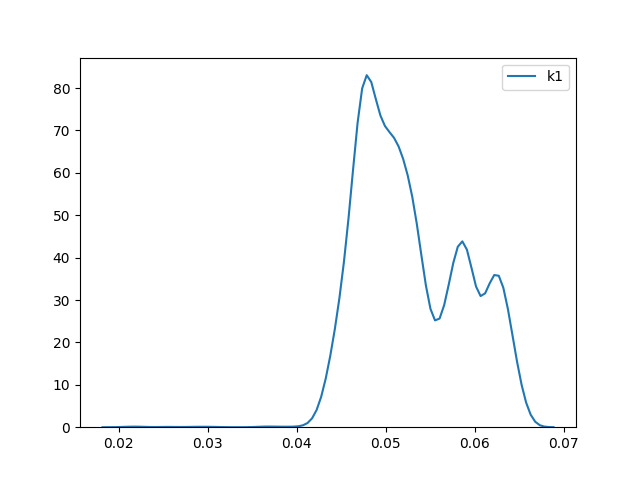
\includegraphics[clip=true]{posterior_after_first_phase_k1.png}}
     \label{fig:posterior_k1_1} }
    & 
    \subfigure[] {\scalebox{.4}{
    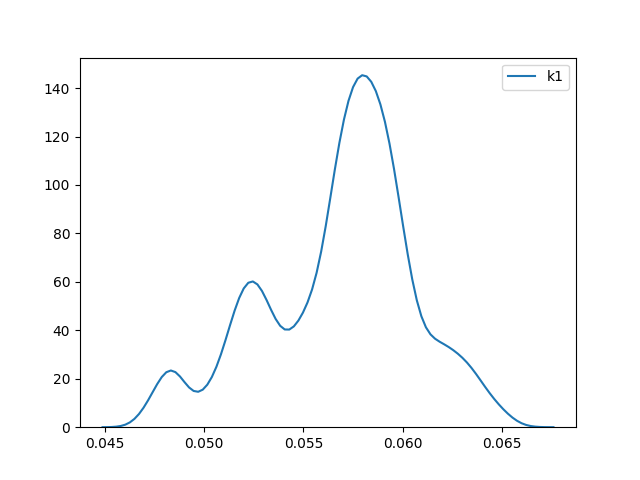
\includegraphics[clip=true]{posterior_after_second_phase_k1.png}}
    \label{fig:posterior_k1_2} }
    \\
    \subfigure[] {\scalebox{0.4}{
     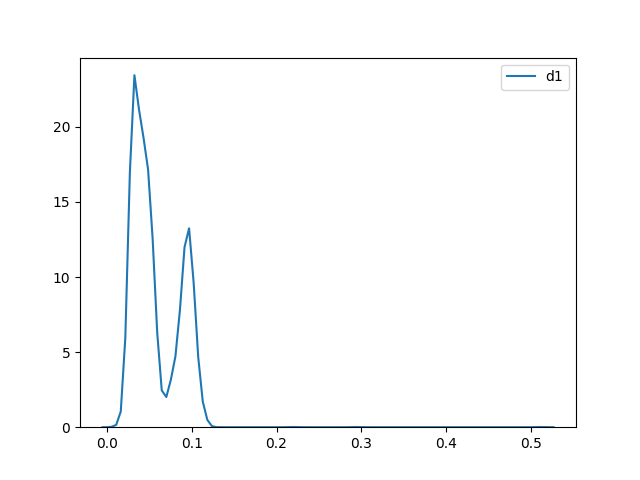
\includegraphics[clip=true]{posterior_after_first_phase_d1.png}}
     \label{fig:posterior_d1_1} }
    & 
    \subfigure[] {\scalebox{.4}{
    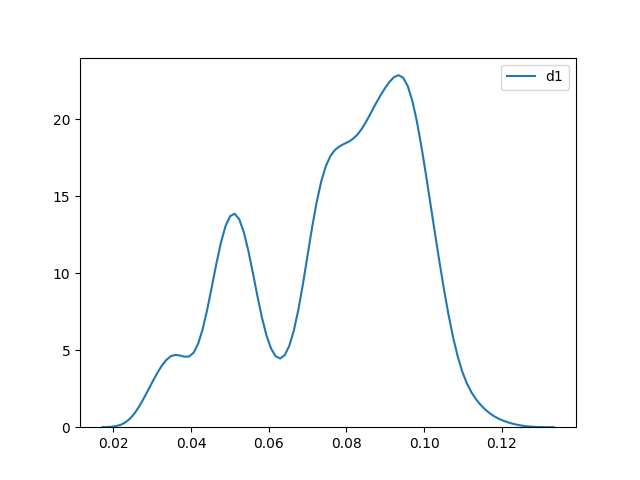
\includegraphics[clip=true]{posterior_after_second_phase_d1.png}}
    \label{fig:posterior_d1_2} }
    \\
    \subfigure[] {\scalebox{0.4}{
     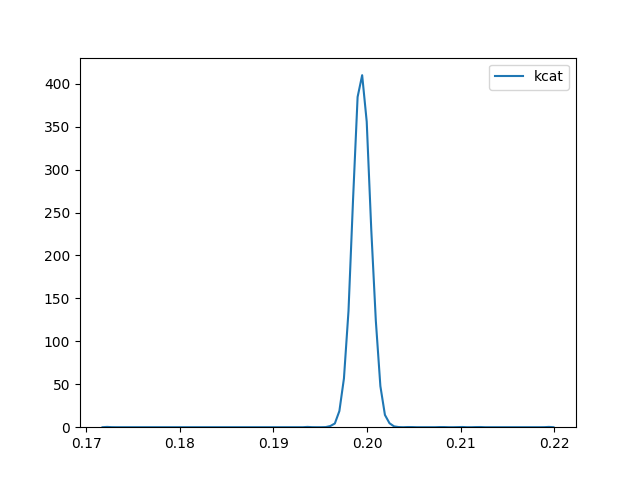
\includegraphics[clip=true]{posterior_after_first_phase_kcat.png}}
     \label{fig:posterior_kcat_1} }
    & 
    \subfigure[] {\scalebox{.4}{
    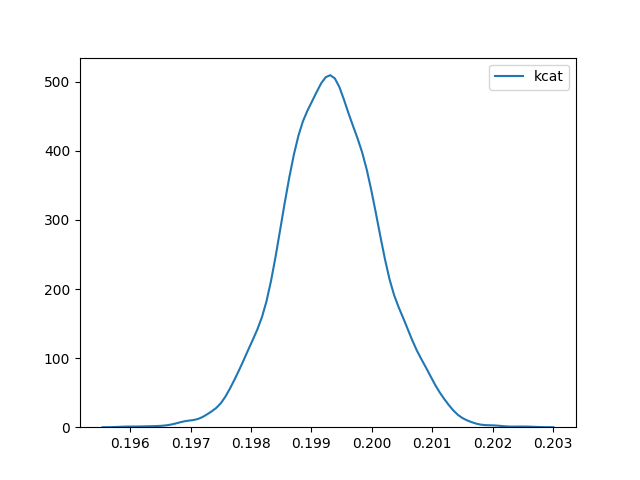
\includegraphics[clip=true]{posterior_after_second_phase_kcat.png}}
    \label{fig:posterior_kcat_2} }
    \\
  \end{tabular}
    \caption{Posteriori estimada de parâmetros após primeira etapa (à 
    esquerda) e segunda etapa (à direita) da geração de amostra da 
    posteriori. Podemos observar nesta figura que a amostra dos 
    parâmetros de fato convergiu para os valores próximos aos que 
    utilizamos para a geraçãoo das observações.}
  \label{fig:posteriori_parameters} 
\end{figure}

\subsubsection{Seleção de modelos em uma instância conhecida}
Neste experimento, nos propomos a reproduzir os resultados encontrados 
por Vyshemirsky e Girolami em~\cite{Vyshemirsky2008}. Neste 
experimento, observações de um modelo funcional são geradas de maneira
similar ao que fizemos no experimento anterior. Além deste modelo, são
criados outros três modelos e então se estima $\log p (D | M)$ para cada 
um deles.

\begin{figure}[ht]
    \begin{center}
    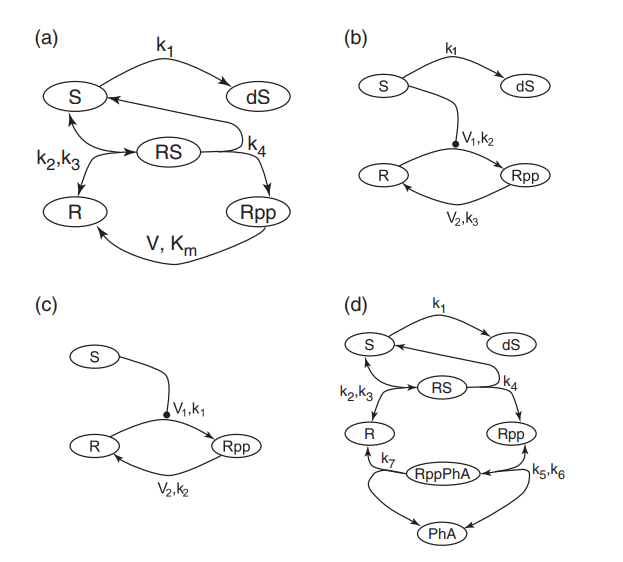
\includegraphics[width=0.65\linewidth]{Vyshemirsky_models.png}
    \caption{Um conjunto de quatro modelos funcionais. Extraído de
        Vyshemirsky e Girolmi~\cite{Vyshemirsky}. Os modelos 1, 2, 3 e
        4 são representados respectivamente pelas letras a, b, c, d.}
    \label{fig:vyshemirsky_models}
    \end{center}

\end{figure}

A figura~\ref{fig:vyshemirsky_models} apresenta os modelos que serão
avaliados neste experimento. O modelo 1 é utilizado para a geração dos
dados; o modelo 2 é uma versão simplificada do modelo 1; o modelo 3 é
um modelo significantemente diferente dos outros; e, por fim, o modelo 4
é uma versão complexa do modelo 1. 

Os resultados obtidos Vyshemirsky e Girolami são apresentados na 
tabela~\ref{tab:vyshemirsky} e indicam que a ordem, por qualidade de 
modelos, é modelo 1 $\prec$ modelo 4 $\prec$ modelo 2 $\prec$ modelo 3. 
Entretanto, como também apresentado na mesma tabela, os resultados que 
obtivemos com SigNetMS implicam na ordenação de qualidade modelo 1 
$\prec$ modelo 4 $\prec$ modelo 3 $\prec$ modelo 2. Acreditamos que esta 
diferença pode ter ocorrido porque na metodologia apresentada por 
Vyshemirsky, a amostragem de $\theta | D, t$ é feita diretamente com o 
algoritmo MCMC populacional, diferente da metodologia empregada pelo 
BIBm e implementada no SigNetMS, que precisa de duas etapas de 
Metropolis-Hastings adaptativas anteriores ao MCMC populacional. Além
disso, ainda estamos repetindo este experimento variando parâmetros dos
algoritmos de Metropolis-Hastings e também removendo as primeiras 
etapas da amostragem, o que pode deixar nossos resultados similares ao
de Vyshemirsky ou indicar erros em nossa implementação.

\begin{table}[ht!]
    \caption{Estitiva de $\log p(D | M)$ obtida para o experimento desta
    seção.}
    \label{tab:vyshemirsky}
    \begin{center}
    \smallskip
    \begin{tabular} {c | c c c c}
        \toprule
        Metodologia & Modelo 1 & Modelo 2 & Modelo 3 & Modelo 4\\
        \hline
        Vyshemirsky e Girolami & 45,8 & 29,2 & -1.1 & 34,8 \\
        SigNetMS &               71,1 & -8,0 &  0.29 & 4.99 \\
        \bottomrule
    \end{tabular}
    \end{center}
\end{table}

\section{Atividades futuras}
Nos próximos dias após a submissão deste relatório, pretendemos dar 
sequência aos experimentos com estimação de verossimilhança marginal 
para garantir que possuímos uma métrica que pode ser utilizada para a
seleção de modelo. Isso nos permitirá, em pouco tempo, construir 
exemplos pequenos em que a nossa metodologia pode ser testada; assim,
pretendemos fazer o exame de qualificação deste projeto junto ao 
Departamento de Ciência da Computação do Instituto de Matemática e 
Estatística da Universidade de São Paulo. Além disso, em um curto prazo,
pretendemos implementar também uma função de custo baseada no critério
de informação AIC; acreditamos que esta tarefa será mais simples do que
previmos na proposta de trabalho, pois esta função de custo é 
consideravelmente mais simples do que o critério utilizado na 
metodologia BIBm.

Como próximo passo, pretendemos iniciar a estruturação do banco de dados 
que será utilizado como base para modificação dos modelos funcionais. 
Após a estruturação, devemos popular o banco com dados reais de diversas 
linhagens de células humanas como HEK293, HaCat, E6E7-Keratinocytes,
Erwing Sarcoma, Nerublastoma, PC12; também células Y1 de camundongos; e
células teóricas simples que serão usadas para testes.

O próximo passo será implementar no arcabouço {\em featsel} uma nova
função de custo para modelos funcionais que funcionará como um 
\foreignword{wrapper} do SigNetMS, chamando este programa para calcular 
$p (D | M)$. Além disso, esta função de custo deve ser capaz de de
conectar o arcabouço com o banco de dados, o que permitirá criar 
representações no formato SBML dos modelos que serão avaliados pelo 
SigNetMS. 

Em seguida, vamos testar a metodologia em 
\foreignword{toy models}, o que será importante para definirmos 
algoritmos de busca que vão decidir como percorrer o espaço de modelos
funcionais; estes algoritmos devem, por exemplo, ser otimizados para 
evitar recálculos, dado que a função de custo SigNetMS deve ser cara
computacionalmente. Além de \foreignword{toy models}, podemos utilizar 
vias de sinalização que possuem modelos funcionais bem conhecidos para 
testar nossa metodologia. Por exemplo, podemos remover interações de um 
modelo funcional criando um modelo incompleto, e rodando nosso 
algoritmo, devemos obter novamente o modelo inicial.

Assim que testadas a função de custo e os algoritmos para o 
percorrimento de espaço de soluções, poderemos enfim aplicar a nossa 
metodologia em linhagens celulares reais, como as descritas 
anteriormente. Para esta etapa, poderemos fazer contribuições para 
colegas do Laboratório Especial de Toxinologia Aplicada que estudam
vias de sinalização celular em células cancerígenas.

Além disso, ao longo do próximo ano devemos elaborar a dissertação e 
fazer a defesa deste trabalho para obtenção do título de mestre pelo
beneficiário.

\subsection{Descrição de atividades}
\begin{itemize}
    \item{\bf Atividade 1:} Finalização dos experimentos com SigNetMS.
    \item{\bf Atividade 2:} Estudo do critério de informação AIC.
    \item{\bf Atividade 3:} Implementação de uma nova função de custo,
        baseado no critério de informação AIC.
    \item{\bf Atividade 4:} Testes das funções de custo com 
        {\em toy models} e modelos funcionais conhecidos.
    \item{\bf Atividade 5:} Exame de qualificação para o mestrado.
    \item{\bf Atividade 6:} Criação do banco de dados que permita
        armazenar interações retiradas de bancos de dados de iteratomas.
    \item{\bf Atividade 7:} Estudo de bancos de dados de cinética 
        química como o SABIO-RK~\cite{doi:10.1093/nar/gkr1046} e 
        BRENDA~\cite{doi:10.1093/nar/gkh081}.
    \item{\bf Atividade 8:} Reestruturação do banco de dados de interações para 
        armazenar também constantes de velocidade.
    \item{\bf Atividade 9:} Estabelecer leis de cinética adequadas para natureza das
        espécies químicas envolvidas.
    \item{\bf Atividade 10:} Integração do banco de dados de interações 
        criado ao CeTICSdb.
    \item{\bf Atividade 11:} Criação de uma nova função de custo no 
        {\em featsel} que deve ser um wrapper do SigNetMS
    \item{\bf Atividade 12:} Criação de outra nova função de custo no
        {\em featsel} que deve utilizar como base o critério AIC para 
        avaliar modelos.
    \item{\bf Atividade 13:} Criações de novos algoritmos de seleção de
        caracteŕísticas para seleção de modelos.
    \item{\bf Atividade 14:} Testes da metodologia com modelos 
        funcionais conhecidos.
    \item{\bf Atividade 15:} Aplicação da metodologia em vias de 
        sinalização de linhagens de células tumorais.
    \item{\bf Atividade 16:} Escrita da dissertação.
    \item{\bf Atividade 17:} Defesa de mestrado.
\end{itemize}

\subsection{Cronograma proposto}

Um cronograma para o período de dezembro de 2018 até dezembro de 2019
é apresentado pela tabela~\ref{tab:cronograma}.

% 1. Finalização de experimentos e testes do SigNetMS
% 2. EQM
% 3. Estruturação do bancos de dados
% 4. População do BD com dados reais das linhagens
%   - Y1
%   - HEK293
%   - HaCat
%   - E6E7-keratinocytes
%   - Erwing Sarcoma
%   - Neuroblastoma
%   - PC12
%   - ToyModels
% 5. Wrapper do SigNetMS ao featsel
% 6. Testes com toy models
% 7. Aplicação da metodologia em linhagens celulares
% 8. Análise  dos resultados
% 9. Elaboração da dissertação
% 10. Defesa

\begin{table}[ht!]
\caption{Cronograma das próximas atividades do projeto.} 
\label{tab:cronograma}
\begin{center}
\smallskip
\resizebox{\columnwidth}{!}{
\begin{tabular}{c c ccc ccc ccc ccc}
    \toprule
    \small \# atividade / mês & \small Dez.18 & \small Jan.19 & \small Fev.19 & \small Mar.19
                         & \small Abr.19 & \small Mai.19 & \small Jun.19
                         & \small Jul.19 & \small Ago.19 & \small Set.19
                         & \small Out.19 & \small Nov.19 & \small Dez.19
    \\ \hline
    1   
    & \small {\bf x} & \small - & \small - & \small -
    & \small - & \small - & \small - & \small - 
    & \small - & \small - & \small - & \small - & \small - \\ 
    2   
    & \small {\bf x} & \small - & \small - & \small - 
    & \small - & \small - & \small - & \small - 
    & \small - & \small - & \small - & \small - & \small - \\ 
    3   
    & \small - & \small {\bf x} & \small {\bf x} & \small - 
    & \small - & \small - & \small - & \small - 
    & \small - & \small - & \small - & \small -  & \small - \\ 
    4
    & \small - & \small {\bf x} & \small {\bf x} & \small -
    & \small - & \small - & \small - & \small - 
    & \small - & \small - & \small - & \small - & \small - \\ 
    5   
    & \small - & \small - & \small - & \small {\bf x} 
    & \small - & \small - & \small - & \small - 
    & \small - & \small - & \small - & \small - & \small - \\ 

    6   
    & \small - & \small - & \small - & \small {\bf x}
    & \small - & \small - & \small - & \small -
    & \small - & \small - & \small - & \small - & \small - \\ 

    7
    & \small - & \small - & \small - & \small {\bf x}  
    & \small {\bf x} & \small - & \small - & \small -
    & \small - & \small - & \small - & \small - & \small - \\ 

    8
    & \small - & \small - & \small - & \small -  
    & \small {\bf x} & \small - & \small - & \small -
    & \small - & \small - & \small - & \small - & \small - \\ 
    9
    & \small - & \small - & \small - & \small -  
    & \small - & \small {\bf x} & \small {\bf x} & \small -
    & \small - & \small - & \small - & \small - & \small - \\ 
    10
    & \small - & \small - & \small - & \small -  
    & \small - & \small - & \small {\bf x} & \small -
    & \small - & \small - & \small - & \small - & \small - \\ 
    11
    & \small - & \small - & \small - & \small -  
    & \small - & \small - & \small {\bf x} & \small -
    & \small - & \small - & \small - & \small - & \small - \\ 
    12
    & \small - & \small - & \small - & \small -  
    & \small - & \small - & \small - & \small {\bf x}
    & \small - & \small - & \small - & \small - & \small - \\ 
    13
    & \small - & \small - & \small - & \small -  
    & \small - & \small - & \small - & \small {\bf x}
    & \small {\bf x} & \small {\bf x} & \small - & \small - & \small - \\ 
    14
    & \small - & \small - & \small - & \small -  
    & \small - & \small - & \small - & \small -
    & \small - & \small {\bf x} & \small {\bf x} & \small - & \small - \\ 

    15
    & \small - & \small - & \small - & \small -  
    & \small - & \small - & \small - & \small -
    & \small - & \small - & \small - & \small {\bf x} & \small {\bf x} \\ 
    16
    & \small - & \small {\bf x} & \small {\bf x} & \small {\bf x}  
    & \small {\bf x} & \small {\bf x} & \small {\bf x} & \small {\bf x}
    & \small {\bf x} & \small {\bf x} & \small {\bf x} & \small {\bf x} & \small {\bf x} \\ 
    17
    & \small - & \small - & \small - & \small -  
    & \small - & \small - & \small - & \small -
    & \small - & \small - & \small - & \small - & \small {\bf x} \\ 

    \bottomrule
\end{tabular}
}
\end{center}
\end{table}

\subsection{Outras atividades acadêmicas}
Além das atividades descritas na seção anterior, o beneficiário deverá
participar de outros eventos acadêmicos. Primeiro, entre os dias 
7 e 11 de janeiro de 2019, o beneficiário participará da XIV Escuela de
Verano en Matemáticas Discretas, em Valparaíso - Chile; a inscrição
do beneficiário neste evento já foi aceita e a participação deferida 
pela FAPESP. 

Também pretendemos apresentar os resultados deste trabalho
em conferências internacionais e nacionais. Em eventos nacionais, 
devemos apresentar pôsteres na conferência X-meeting e também na Reunião
Científica Anual do Instituto Butantan. Também pretendemos participar
do International Conference in Systems Biology (ICSB).
% Santiago (outorgado pela FAPESP)
% Apresentar resultados em conferência internacional (ICSB)
% Apresentar resultados em outra conferencia nacional (X-meeting e RCA)

\addcontentsline{toc}{section}{Referências}
\bibliographystyle{unsrt} 
\bibliography{bib-relatorio}
\end{document}


